\chapter{Flexible Variational Auto-Encoders}

\section{A Review of Variational Auto-Encoders}
\label{sec:vae}
As we did with diffusion models in \cref{ch:diffusion}, we will start by reviewing variational auto-encoders, or VAEs~\citep{kingma2013auto,rezende2014stochastic}, as unconditional generative models. We will then explain a conditional variant in \cref{sec:conditional-vae}. Like a diffusion model a variational auto-encoder is trained, using samples from a data distribution $\pdata(\rvx)$, to approximate $\pdata(\rvx)$. Given a variational auto-encoder with parameters $\theta$, we will denote the distribution it parameterises $p_\theta(\rvx)$. The key feature of a VAE is that it breaks the process of generating data into two steps: in the first step a VAE samples a latent variable $\rvz$ from a ``prior'' distribution $p_\theta(\rvz)$. The prior distribution can be fixed, \eg a unit Gaussian, or can have learnable parameters that are included in $\theta$. In the second step, the VAE parameterises a ``likelihood'' $p_\theta(\rvx|\rvz)$. This can be, \eg, a Gaussian for continuous data~\citep{kingma2013auto} or a categorical for discrete data~\citep{child2020very}, with parameters output in either case by a neural network as a function of $\rvz$. We can therefore write the parameterised distribution $p_\theta(\rvx)$ as the marginal of $p_\theta(\rvx|\rvz)$ over the latent variable $\rvz$,
% that is $p_\theta(\rvx) = \int p_\theta(\rvx|\rvz) p_\theta(\rvz) \mathrm{d}\rvz$.
\begin{equation} \label{eq:vae-marginal}
p_\theta(\rvx) = \int p_\theta(\rvx|\rvz)p_\theta(\rvz) \mathrm{d}\rvz.
\end{equation}
Even if both the prior $p_\theta(\rvz)$ and likelihood $p_\theta(\rvx|\rvz)$ are simple distributions, the marginal $p_\theta(\rvx)$ can be complex since the likelihood can be given by an arbitrarily complex function of $\rvz$.

As we discussed for diffusion models in \cref{ch:diffusion}, an ideal training objective would maximise the data likelihood $p_\theta(\rvx)$ averaged over all training examples since this corresponds to learning parameters which maximise the likelihood of the dataset under the learned distribution. The required marginalisation in \cref{eq:vae-marginal}, however, means that directly estimating the data likelihood is intractable. Therefore, as for diffusion models, we instead derive a training objective that lower-bounds the data likelihood. Starting by taking an expectation of the log of the data likelihood in \cref{eq:vae-marginal}, we can obtain a lower-bound using a proposal distribution $q_\phi(\rvz|\rvx)$ which can be given by a neural network with parameters $\phi$: % our objective can be converted to the log of an expectation over $q_\phi(\rvz)$:
\begin{align}
    \EX_{\pdata(\rvx)} \left[ \log p_\theta(\rvx) \right] &= \EX_{\pdata(\rvx)} \left[ \log \int p_\theta(\rvx|\rvz)p_\theta(\rvz) \mathrm{d}\rvz \right] \\
    &= \EX_{\pdata(\rvx)} \left[ \log \int p_\theta(\rvx|\rvz) \frac{p_\theta(\rvz)}{q_\phi(\rvz|\rvx)} q_\phi(\rvz|\rvx) \mathrm{d}\rvz \right] \\
    &= \EX_{\pdata(\rvx)} \left[ \log \EX_{q_\phi(\rvz|\rvx)} \left[ p_\theta(\rvx|\rvz) \frac{p_\theta(\rvz)}{q_\phi(\rvz|\rvx)} \right] \right]. \label{eq:vae-marginal-is}
\end{align}
Ideally we would be able to obtain an unbiased estimate of this objective. Due to the logarithm operator outside an intractable expectation this is not feasible but, using Jensen's inequality, we can obtain a training objective that lower bounds it by switching their order: 
\begin{align}
    \gL(\theta, \phi) := \EX_{\pdata(\rvx)q_\phi(\rvz|\rvx)} \left[ \log p_\theta(\rvx|\rvz) + \log \frac{p_\theta(\rvz)}{q_\phi(\rvz|\rvx)} \right] \leq \EX_{\pdata(\rvx)} \left[ \log p_\theta(\rvx) \right].
    \label{eq:vae-objective}
\end{align}
This lower-bound can be stochastically estimated by sampling data $\rvx$ and then sampling $\rvz$ from $q_\phi(\rvz|\rvx)$ and evaluating the terms inside the expectation with that given $\rvz$. Since $q_\phi(\rvz|\rvx)$ ``encodes'' data $\rvx$ into latent variables $\rvz$ we will from now on refer to it as the encoder. The tightness of this lower-bound is strongly dependent on how ``good'' the encoder $q_\phi(\rvz|\rvx)$ is, and we can make this insight clear by rewriting \cref{eq:vae-objective} as
\begin{equation}
    \gL(\theta, \phi) := \EX_{\pdata(\rvx)} \left[ \log p_\theta(\rvx) - \kl{q_\phi(\rvz|\rvx)}{p_\theta(\rvz|\rvx)} \right].
\end{equation}
This formulation reveals that the lower-bound is tight if and only if the proposal $q_\phi(\rvz|\rvx)$ is equal to the generally intractable posterior $p_\theta(\rvz|\rvx)$ causing the KL divergence term to be zero. Fortunately, maximising this objective with respect to $\theta$ and $\phi$ will optimise the proposal parameters $\phi$ to better match the intractable posterior as well as optimising $\theta$ to increase the model likelihood, and so it is possible to train both $\theta$ and $\phi$ with a unified objective. The full optimisation objective is thus
\begin{align}
    \argmin_{\theta,\phi} \gL(\theta, \phi).
\end{align}

\section{A Review of Hierarchical Variational Auto-Encoders}
\label{sec:hierarchical-vae}
\begin{figure}
    \centering
    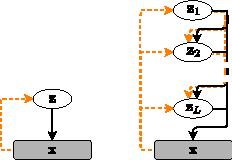
\includegraphics[width=0.5\textwidth]{figs/thesis/vae-vs-hierarchical-vae.pdf}
    \caption{A comparison of the dependency structure of a ``standard'' VAE (left) with that of a top-down hierarchical VAE (right). For each, we show the dependencies of each variable in the encoder's distribution though dashed orange lines and the dependencies of each variable in the prior and decoder's distributions with solid black lines.}
    \label{fig:vae-vs-hierarchical-vae}
\end{figure}
A hierarchical VAE~\citep{gregor2015draw,kingma2016improving,sonderby2016ladder,klushyn2019learning} is a special case of a VAE which has latent variables $\rvz$ with a particular structure. In particular, $\rvz$ is partitioned into $L$ disjoint groups, $\rvz_1,\ldots,\rvz_L$. The prior $p_\theta(\rvz) = p_\theta(\rvz_1,\ldots,\rvz_L)$ and encoder $q(\rvz|\rvx) = q_\phi(\rvz_1,\ldots,\rvz_L|\rvx)$ are then factorised to enable them to represent structured distributions over $\rvz$. Exactly how these distributions are factorised is a design choice but the hierarchical VAEs that we will consider in this thesis are ``top-down'' meaning that they factorise the prior and the encoder distributions in the same order~\citep{vahdat2020nvae,child2020very}:
\begin{equation}
    p_\theta(\rvz) = \prod_{l=1}^L p_\theta(\rvz_l|\rvx,\rvz_{<l}) \quad \text{and} \quad q_\phi(\rvz|\rvx) = \prod_{l=1}^L q_\phi(\rvz_l|\rvx,\rvz_{<l})
\end{equation}
where $\rvz_{<l}$ is the set of all latent variable groups from $\rvz_1$ (inclusive) to $\rvz_{l}$ (exclusive) if $l > 1$ and is null otherwise. We show this dependency structure graphically in \cref{fig:vae-vs-hierarchical-vae}.

Hierarchical VAEs are closely related to diffusion models, and in fact diffusion models can be interpreted as a special case of a hierarchical VAE. Given an increasing sequence of noise standard deviations $\sigma(1),\ldots,\sigma(L)$, we can present a variance-exploding diffusion model as a top-down hierarchical VAE with an encoder
\begin{align}
    q(\rvz|\rvx) &= q(\rvz_1|\rvx) \prod_{l=2}^L q(\rvz_l | \rvx, \rvx_{l-1}) \\
    &= \gN( \rvz_1 ; \rvx, \sigma(L)^2 \mI ) \prod_{l=2}^L \gN( \rvz_l | \mu^l_Q(\rvz_{l-1}, \rvx), {\sigma_Q^l}^2 \mI )
\end{align}
where $\mu^l_Q(\rvz_{l-1}, \rvx) := \mu_Q(\rvz_{l-1}, \rvx; \rho, \sigma)$ and $\sigma^l_Q := \sigma_Q(\rho, \sigma)$ with $\mu_Q$ and $\sigma_Q$ as defined in \cref{eq:mu-q,eq:sigma-q} and $\rho := \sigma(L-l)$, $\sigma := \sigma(L+1-l)$. Note that this encoder has no learnable parameters, i.e. $\phi$ is empty. In the setting described in \cref{sec:diffusion-likelihood}, a diffusion model then approximates each $p_\theta(\rvz_l|\rvz_{<l})$ as a Gaussian. The use of a fixed encoder and Gaussian forms enables many tricks to be used in diffusion models that are not possible for most variational auto-encoders. In particular, diffusion models allow an efficient training objective that can subsample the layer $l$ and compute a loss estimate for a data point using a single value of $l$, whereas a the loss for a hierarchical VAE must typically be summed over all layers for every data point. The diffusion framework also enables weighting of the loss to improve perceptual quality, as we described in \cref{sec:diffusion-perceptual-quality}, and the use of ODEs or SDEs for improved performance at test-time versus explicitly sampling from each $p_\theta(\rvz_l|\rvz_{<l})$.
A major advantage of VAEs, on the other hand, is the learnable encoder which makes it theoretically possible to learn fast and effective procedures for sampling datapoints other than simply progressively removing Gaussian noise. 

Although diffusion models currently dominate at the core tasks of e.g. image and video generation~\citep{esser2024scaling,brooks2024video}, variants of VAEs are used for other purposes including as tools to compress data $\rvx$ into latent variables $\rvz$ that are then modelled with other techniques like diffusion models. We also note that the two-stage diffusion model~\cref{sec:2sdm-2sdm-method} could be interpreted as a form of variational auto-encoder in which the prior $p_\theta(\rvz)$ and decoder $p_\theta(\rvx|\rvz)$ are both parameterised by diffusion models and the encoder is frozen to a pretrained value. We believe that it is valuable to demonstrate that flexible generative modelling works within the variational auto-encoder framework and for these reasons, and to provide more reason to believe that it could apply to other generative modelling frameworks in addition.

\section{A Review of Conditional Variational Auto-Encoders}
\label{sec:conditional-vae}

% \section{Conditional Variational Auto-Encoders}
Our focus in this thesis is on conditional, rather than unconditional, generative models. In the setting we consider we want to approximate the conditional distribution $p_\theta(\rvx|\rvy)$ and at training time have access to either a joint distribution $p_\theta(\rvx,\rvy)$ or a dataset of $(\rvx, \rvy)$ pairs that we can use to approximate the joint distribution.

In order to match the distribution modeled by a VAE to such a conditional distribution, at least one of the prior or decoder should be made conditional on $\rvz$. To cover all cases, we will write both as conditional on $\rvy$. That is, we will denote the prior distribution of a conditional VAE $p_\theta(\rvz|\rvy)$ and the decoder's distribution as $p_\theta(\rvx|\rvy,\rvz)$. The encoder may in principle also be made conditional on $\rvy$, but that is not the case for any of the generative models considered in this thesis and so we will continue to write it as $q_\phi(\rvz|\rvx)$. See \cref{tab:vae_components} for a summary of these differences. The distribution modelled is, as before, obtained by marginalising over $\rvz$ as
\begin{equation} \label{eq:vae-marginal}
p_\theta(\rvx|\rvy) = \int p_\theta(\rvx|\rvy,\rvz)p_\theta(\rvz|\rvy) \mathrm{d}\rvz
\end{equation}
and the training objective for both $\theta$ and $\phi$ is
\begin{equation}
    \gL(\rvx, \rvy, \theta, \phi) = \EX_{q_\phi(\rvz|\rvx)} \left[ \log p_\theta(\rvx|\rvy,\rvz) + \log \frac{p_\theta(\rvz|\rvy)}{q_\phi(\rvz|\rvx)} \right].
\end{equation}

To understand the properties of VAEs, we now take a look at a few ways to decompose this training objective. One is to separate the objective into a reconstruction loss and a KL divergence:
\begin{align}
    \gL(\rvx, \rvy, \theta, \phi) &= \underbrace{\EX_{q_\theta(\rvz|\rvx)} \left[ \log p_\theta(\rvx|\rvz) \right]}_\text{reconstruction loss} + \underbrace{\kl{q_\phi(\rvz|\rvx)}{p_\theta(\rvz)}}_\text{KL divergence},
\label{eq:marginal-is}
\end{align}
The reconstruction loss encourages the encoder and decoder to be learned such that little information is lost if we map a data point $\rvx$ to latent space and back. The KL divergence penalises differences between the encoder's proposal distribution and the prior distribution.

If we consider the expectation of the objective over the data distribution, we can get furhter insight by separating terms into the entropy of the target distribution and a KL divergence:
\begin{align}
  \EX_{\pdata(\rvx,\rvy)} &\left[ \mathcal{L}(\rvx, \rvy, \theta, \phi) \right] \\
  =& \EX_{\pdata(\rvx,\rvy)} \EX_{q_\phi(\rvz|\rvx)} \left[ \log \pdata(\rvx|\rvy) + \log \frac{p_\theta(\rvx,\rvz|\rvy)}{q_\phi(\rvz|\rvx)\pdata(\rvx|\rvy)} \right]\\
    =& -\mathcal{H}\left[ \pdata(\rvx|\rvy) \right] - \kl[\big] { \pdata(\rvx|\rvy) q_\phi(\rvz|\rvx) }{ p_\theta(\rvx,\rvz|\rvy) }. \label{eq:elbo-kl-joints}
\end{align}
where $p_\theta(\rvx,\rvz|\rvy)$ is the joint distribution defined as $p_\theta(\rvx|\rvy,\rvz)p_\theta(\rvz|\rvy)$ and $\mathcal{H}\left[ \pdata(\rvx|\rvy) \right]$ is the differential entropy of the target distribution. While the differential entropy is not guaranteed to be finite in general, it always will be when $\rvx$ is finite, as is common for pixel values in the image and video domains. Since the KL divergence is always non-negative, our training objective is upper-bounded by the differential entropy. Additionally, the KL-divergence is in the direction which causes mass-covering behaviour~\citep{bishop2006pattern} and so we can expect the learned distribution $p_\theta(\rvx|\rvy)$ to assign probability broadly over the data distribution $\pdata(\rvx|\rvy)$, with any missed modes being heavily penalised.

% \begin{table}[t]
% \centering
% % \begin{tabular}{c|c|c|c}
% %  & Prior & Decoder & Encoder \\ 
% % \hline
% % Unconditional VAE & \( p_\theta(\rvz) \) & \( p_\theta(\rvx|\rvz) \) & \( q_\phi(\rvz|\rvx) \) \\
% % Conditional VAE & \( p_\theta(\rvz|\rvy) \) & \( p_\theta(\rvx|\rvy,\rvz) \) & \( q_\phi(\rvz|\rvx) \) \\
% % \end{tabular}
% \begin{tabular}{l|ll|ll}
%  & \multicolumn{2}{c|}{Unconditional} & \multicolumn{2}{c}{Conditional} \\ 
% \cline{2-5}
% & Notation & Definition & Notation & Definition \\ 
% \hline
% Prior & \( p_\theta(\rvz) \) & primitive  & \( p_\theta(\rvz|\rvy) \) & primitive  \\
% Decoder & \( p_\theta(\rvx|\rvz) \) & primitive  & \( p_\theta(\rvx|\rvy,\rvz) \) & primitive \\
% Encoder & \( q_\phi(\rvz|\rvx) \) & primitive  & \( q_\phi(\rvz|\rvx) \) & primitive \\
% Predictive & \( p_\theta(\rvx) \) & \( \int p_\theta(\rvx|\rvz)p_\theta(\rvz) \mathrm{d}\rvz \)  & \( p_\theta(\rvx|\rvy) \) & \( \int p_\theta(\rvx|\rvy,\rvz)p_\theta(\rvz) \mathrm{d}\rvz \) \\
% \end{tabular}
% \caption{Comparison of our notation for distributions relating to an unconditional versus a conditional VAE. The prior, decoder, and encoder distributions are primitives directly parameterised by neural networks. The predictive distribution, which we train to match a target distribution, is defined via a marginalisation.}
% \label{tab:vae_components}
% \end{table}



% \section{Hierarchical Variational Auto-Encoders} \label{sec:hierarchical-vae}
% In this section we introduce the conditional version of a hierarchical VAE, but note that our description can be transferred to the unconditional setting by removing any dependencies on $\rvy$ or setting $\rvy$ to null. A (conditional) hierarchical VAE~\citep{gregor2015draw,kingma2016improving,sonderby2016ladder,klushyn2019learning} is a (conditional) VAE in which the latent variables $\rvz$ have a particular structure. In particular, $\rvz$ is partitioned into $L$ disjoint groups, $\rvz_1,\ldots,\rvz_L$. The prior $p_\theta(\rvz|\rvy) = p_\theta(\rvz_1,\ldots,\rvz_L|\rvy)$ and encoder $q(\rvz|\rvx,\rvy) = q_\phi(\rvz_1,\ldots,\rvz_L|\rvx,\rvy)$ are then factorised to enable them to represent structured distributions over $\rvz$. How these distributions are factorised is a design choice.
% The hierarchical VAEs that we will consider in this thesis are ``top-down'' meaning that they factorise the prior and the encoder distributions in the same order~\citep{vahdat2020nvae,child2020very}:
% \begin{equation}
%     p_\theta(\rvz) = \prod_{l=1}^L p_\theta(\rvz_l|\rvx,\rvz_{<l}) \quad \text{and} \quad q_\phi(\rvz|\rvx) = \prod_{l=1}^L q_\phi(\rvz_l|\rvx,\rvz_{<l})
% \end{equation}
% where $\rvz_{<l}$ is the set of all latent variable groups from $\rvz_1$ (inclusive) to $\rvz_{l}$ (exclusive) if $l > 1$ and is null otherwise. We show this dependency structure graphically in \cref{fig:vae-vs-hierarchical-vae}.

% \begin{figure}
%     \centering
%     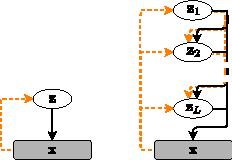
\includegraphics[width=0.5\textwidth]{figs/thesis/vae-vs-hierarchical-vae.pdf}
%     \caption{A comparison of the dependency structure of a ``standard'' VAE (left) with that of a top-down hierarchical VAE (right). For each, we show the dependencies of each variable in the encoder's distribution though dashed orange lines and the dependencies of each variable in the prior and decoder's distributions with solid black lines. Note that, in the case of a conditional VAE, there are additional dependencies of all prior and decoder distributions on $\rvy$, which we do not show.}
%     \label{fig:vae-vs-hierarchical-vae}
% \end{figure}
